\documentclass[24pt]{beamer}
\usepackage[utf8]{inputenc}
\usepackage[utf8]{vietnam}
\usepackage{amsmath}
\usepackage{amsfonts}
\usepackage{amssymb}
\usepackage{graphicx}
\usepackage{multimedia}
\usepackage{tikz}
\usetikzlibrary{positioning}
\usetikzlibrary{arrows}
\usetikzlibrary{decorations.markings}
\usepackage{xcolor}
\usepackage{utopia} %font utopia imported
\usepackage{siunitx}
\usepackage[american,cuteinductors,smartlabels]{circuitikz}
\usepackage{ragged2e}
\usepackage{etoolbox}

\mode<beamer>{\usetheme{CambridgeUS}}

\usecolortheme{default}

\usepackage{hyperref}
\hypersetup{pdfpagemode=FullScreen} %mode FullScreen with beamer

\apptocmd{\frame}{}{\justifying}{} % Allow optional arguments after frame.

\usepackage{comment}

\makeatletter
\let\insertuniversity\relax
\newcommand\universitytitle{TRƯỜNG ĐH}

\let\insertclass\relax
\newcommand\classtitle{Lớp}

\let\insertcourse\relax
\newcommand\coursetitle{Môn học}

\mode<all>
{
  \newcommand\university[1]{\def\insertuniversity{#1}}
  
  \newcommand\class[1]{\def\insertclass{#1}}
  
  \newcommand\course[1]{\def\insertcourse{#1}}
  \titlegraphic{}
}

\defbeamertemplate*{title page}{supdefault}[1][]
{
  \begingroup
    \centering
    \ifx\insertuniversity\relax\relax\else
    \begin{beamercolorbox}[sep=2pt,center,#1]{author}
      \hspace{-.15cm}\scriptsize\universitytitle~\insertuniversity
    \end{beamercolorbox}\fi
    
    \begin{beamercolorbox}[sep=8pt,center,#1]{title}
      \usebeamerfont{title}\normalsize\inserttitle\par%
      \ifx\insertsubtitle\@empty\relax%
      \else%
        \vskip0.25em%
        {\usebeamerfont{subtitle}\usebeamercolor[fg]{subtitle}\insertsubtitle\par}%
      \fi%     
    \end{beamercolorbox}%
    \vskip.5em\par

    \vspace{-.4cm}
    \ifx\insertcourse\relax\relax\else
    \begin{beamercolorbox}[sep=6pt,center,#1]{author}
      \usebeamerfont{author}\footnotesize\coursetitle:~\insertcourse
    \end{beamercolorbox}\fi

    \vspace{-.3cm}
    \ifx\insertclass\relax\relax\else
    \begin{beamercolorbox}[sep=6pt,center,#1]{author}
      \usebeamerfont{author}\footnotesize\classtitle:~\insertclass
    \end{beamercolorbox}\fi

    \vspace{-.3cm}
    \begin{beamercolorbox}[sep=6pt,center,#1]{author}
      \usebeamerfont{author}\hspace{-.23cm}\footnotesize\insertauthor
    \end{beamercolorbox}
    %\begin{beamercolorbox}[sep=8pt,center,#1]{institute}
      %\usebeamerfont{institute}\insertinstitute
    %\end{beamercolorbox}
    \vspace{-.4cm}
    \begin{beamercolorbox}[sep=8pt,center,#1]{date}
      \usebeamerfont{date}\footnotesize\insertdate
    \end{beamercolorbox}\vskip0.5em
    {\usebeamercolor[fg]{titlegraphic}\inserttitlegraphic\par}
  \endgroup
  \vfill
}
\setbeamertemplate{title page}[supdefault][colsep=-4bp,rounded=true,shadow=\beamer@themerounded@shadow]\makeatother

%Title page
\title[Động cơ điện một chiều]{\emph{Chủ đề báo cáo}\\ \hspace{-1cm} Nguyên lí hoạt động, Đặc tính cơ, Các PP khởi động ĐC DC}
\author[Cơ sở Truyền động điện]{GVHD: Hồ Minh Nhị \and Nhóm SVTH: Nhóm 1}
\course{Cơ sở Truyền động điện}
\class{Công nghệ, kỹ thuật điện, điện tử}
\university{KỸ THUẬT -- CÔNG NGHỆ CẦN THƠ}
\date[Nhóm 1]{\today}
%\date[Nhóm 1]{Ngày 24 tháng 08 năm 2016}

%\logo{\includegraphics[height=1.3cm]{logo_ctut.pdf}}

\AtBeginSection[]
{
  \begin{frame}
    \frametitle{Nội dung báo cáo}
    \justifying
    \tableofcontents[currentsection]
  \end{frame}
}
\definecolor{doden}{RGB}{204, 0, 0}
\newcommand{\noibat}[1]{\textcolor{red}{#1}}
\newcommand{\noibatn}[1]{\textcolor{blue}{#1}}
\newcommand{\drawe}{\draw[line width=1.2pt]}
\begin{document}
%http://tex.stackexchange.com/questions/82794/removing-page-number-from-title-frame-without-changing-the-theme
\bgroup
\makeatletter
\setbeamertemplate{footline}
{
  \leavevmode%
  \hbox{%
  \begin{beamercolorbox}[wd=.333333\paperwidth,ht=2.25ex,dp=1ex,center]{author in head/foot}%
    \usebeamerfont{author in head/foot}\insertshortauthor\expandafter\beamer@ifempty\expandafter{\beamer@shortinstitute}{}{~~(\insertshortinstitute)}
  \end{beamercolorbox}%
  \begin{beamercolorbox}[wd=.333333\paperwidth,ht=2.25ex,dp=1ex,center]{title in head/foot}%
    \usebeamerfont{title in head/foot}\insertshorttitle
  \end{beamercolorbox}%
  \begin{beamercolorbox}[wd=.333333\paperwidth,ht=2.25ex,dp=1ex,right]{date in head/foot}%
    \usebeamerfont{date in head/foot}\insertshortdate{}\hspace*{2em}
%    \insertframenumber{} / \inserttotalframenumber\hspace*{2ex} 
    \hspace*{6ex}
  \end{beamercolorbox}}%
  \vskip0pt%
}

\begin{frame}
\titlepage
\end{frame}
\egroup

\setcounter{framenumber}{0}

%--------------------------------------------------------------------------------
%--------------------------------------------------------------------------------
% Danh sách thành viên
\begin{frame}{Danh sách thành viên}
%	\vspace{-1cm}
	\begin{footnotesize}
	\begin{columns}
		\column{0.6\textwidth}
		\begin{enumerate}
			\item Nguyễn Văn Bảy
			\item Nguyễn Văn Đình
			\item Nguyễn Hoàng Hận
			\item Thi Minh Nhựt
			\item Phạm Thanh Quý
			\item Hồ Minh Thành
			\end{enumerate}

		\column{.6\textwidth}
		\begin{enumerate}	% Danh sach tiep theo
			\setcounter{enumi}{6}
			\item Nguyễn Văn Tiến
			\item Liên Thái Trường
			\item Trần Thanh Tú
			\item Bùi Trọng Tuấn
			\item Lư Anh Tuấn
			\item Nguyễn Bá Vọng
		\end{enumerate}
	\end{columns}
	\end{footnotesize}
\end{frame}

%--------------------------------------------------------------------------------
%--------------------------------------------------------------------------------
% Nội dung báo cáo
\begin	{frame}	%Trang muc luc
	\frametitle{Nội dung báo cáo}
	\tableofcontents
\end{frame}

%--------------------------------------------------------------------------------
%--------------------------------------------------------------------------------
% Nguyên lý hoạt động của động cơ DC
\section[Nguyên lý hoạt động]{Nguyên lý hoạt động của động cơ DC}
\begin{frame}{Nguyên lý hoạt động}
	\begin{figure}[!h]
		\begin{center}
			\href{run:video-mophong/Motor-DC.mp4}{\includegraphics[scale=.8]{video-mophong/Motor-DC.jpg}}
		\end{center}
	\end{figure} 
\end{frame}

%--------------------------------------------------------------------------------
%--------------------------------------------------------------------------------
% Đặc tính cơ của động cơ DC
\section{Đặc tính cơ của động cơ DC}
\subsection*{Đặc điểm}
\begin{frame}{Đặc điểm}
	\justifying
	\begin{itemize}
		\item Quan hệ: \noibat{$M(\omega)$} hoặc \noibat{$\omega(M)$}.

		\item ĐC DC kích từ:
	\end{itemize}
			\begin{tabular}{|m{6.5cm}|m{4.5cm}|l}\cline{1-2}		
			\noibat{Song song}, \noibat{độc lập} & \centering{\noibat{Nối tiếp}} & \\ \cline{1-2}
			$\omega$ giảm ít khi $M$ tăng & $\omega$ và $M$ tỉ lệ nghịch & \\ \cline{1-2}
			\end{tabular}
\end{frame}

\subsection*{Phương pháp thay đổi đặc tính cơ}
\begin{frame}{PP thay đổi đặc tính cơ}
\justifying
	\begin{itemize}
		\item Giảm $U_{\text{\textit{phần ứng}}}$.
		\item Thêm $R_{\text{\textit{phụ mạch phần ứng}}}$.
		\item Giảm kích từ.
	\end{itemize}
\end{frame}

\begin{frame}{PP thay đổi đặc tính cơ}
	\vspace{-1.5cm}
	\begin{center}
		\begin{tikzpicture}
			\drawe[->] (0,0) -- (0,5);
			\drawe[->] (0,0) -- (7,0);
			\drawe[dashed, red] (-1,3.5) -- (6.5,2.5);
			\drawe[green] (-1,1.5) -- (6.5,1);
			\drawe[blue] (-1.2,3.75) -- (6.5,1.35);				\drawe[magenta] (-1,4.5) -- (6.5,2.8);
			\draw (8.5,.5) node {\textcolor{green}{\textit{Giảm} $U_{\text{\textit{ư}}}$}};
			\draw (8.5,1.5) node {\textcolor{blue}{\textit{Tăng} $R_{\text{\textit{ph}}}$}};
			\draw (8.5,2.5) node {\textcolor{red}{\textit{Tự nhiên}}};
			\draw (8,3.5) node {\textcolor{magenta}{\textit{Giảm kích từ}}};
			\draw (7,-.5) node {$M$};
			\draw (0,-.5) node {$0$};
			\draw (-.7,5) node {$\omega_m$};
		\end{tikzpicture}
	\end{center}
\end{frame}

%--------------------------------------------------------------------------------
%--------------------------------------------------------------------------------
% Các phương pháp khởi động động cơ DC
\section[Các PP khởi động động cơ DC]{Các phương pháp khởi động động cơ DC}
\subsection*{PP khởi động động cơ DC}
\begin{frame}{PP khởi động}
\justifying
Tìm hiểu PP khởi động cho 2 loại ĐC DC:
	\begin{itemize}
	\justifying
		\item ĐC DC kích từ độc lập.
		\item ĐC DC kích từ nối tiếp.
	\end{itemize}
\end{frame}

%--------------------------------------------------------------------------------
% Khởi động ĐC DC kích từ độc lập
\subsection*{Khởi động ĐC DC kích từ độc lập}
\begin{frame}{Khởi động động cơ DC kích từ độc lập}
	\begin{itemize}
	\justifying
		\item Dùng nguồn có điều khiển.
		\item Dùng nguồn cố định kết hợp biến trở nối tiếp với phần ứng.
	\end{itemize}
\end{frame}

\begin{frame}{Dùng nguồn có ĐK}
	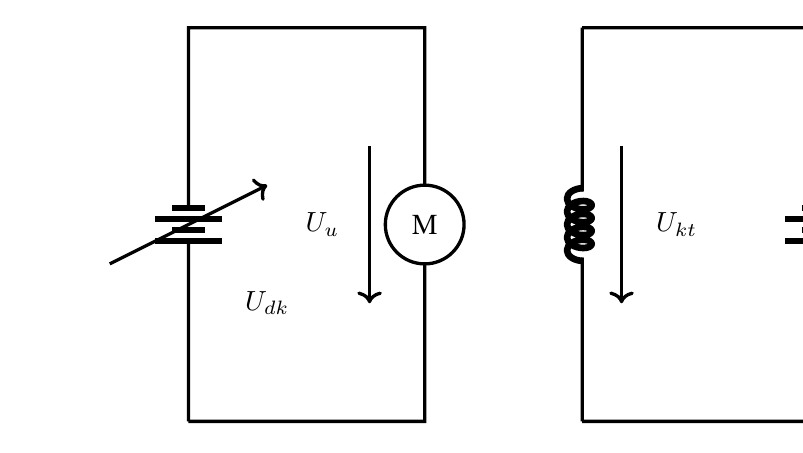
\begin{tikzpicture}
		\begin{circuitikz}
			\drawe (0,0) to [battery] (0,5) to [short] (3,5) to [short] (3,3);
			\drawe (3,2.5) circle (.5) node{M};
			\drawe[->] (2.3,3.5) -- (2.3,1.5);
			\draw (1.7,2.5) node {$U_u$};
			\drawe (3,2) to [short] (3,0) to [short] (0,0);
			
			\drawe (5,0) to [short] (8,0) to [battery] (8,5) to [short] (5,5);
			\drawe (5,0) to [L] (5,5);
			\drawe[->] (5.5,3.5) -- (5.5,1.5);
			\draw (6.2,2.5) node {$U_{kt}$};
			
			\drawe[->] (-1,2) -- (1,3);
			\draw (1,1.5) node {$U_{dk}$};
			
		\end{circuitikz}
	\end{tikzpicture}
\end{frame}

\begin{frame}{Dùng nguồn có ĐK}
	\vspace{-1.4cm}
	\begin{center}
		\begin{tikzpicture}
			\drawe[->] (0,0) -- (0,5.5);
			\drawe[->] (0,0) -- (9.5,0);
			
			\drawe[red] (1,0) -- (1,5);
			\drawe[magenta] (3,0) -- (3,4.5);
			\drawe[dashed, magenta] (7,0) -- (7,4);	
			
			\drawe[draw=blue,-triangle 90,fill=blue] (7,0) -- (5,.5);
			\drawe[blue] (5,.5) -- (3,1);
			\drawe[dashed, draw=blue,-triangle 90,fill=blue] (3,1) -- (5,1);
			\drawe[blue, dashed] (5,1) -- (7,1);	
			\draw[blue, dashed, line width=.6pt] (3,1) -- (0,1.75);
			
			\drawe[draw=blue,-triangle 90,fill=blue] (7,1) -- (5,1.5);
			\drawe[blue] (5,1.5) -- (3,2);
			\drawe[dashed, draw=blue,-triangle 90,fill=blue] (3,2) -- (5,2);
			\drawe[blue, dashed] (5,2) -- (7,2);
			\draw[blue, dashed, line width=.6pt] (3,2) -- (0,2.75);
			
			\drawe[draw=blue,-triangle 90,fill=blue] (7,2) -- (5,2.5);
			\drawe[blue] (5,2.5) -- (3,3);
			\drawe[dashed, draw=blue,-triangle 90,fill=blue] (3,3) -- (5,3);
			\drawe[blue, dashed] (5,3) -- (7,3);
			\draw[blue, dashed, line width=.6pt] (3,3) -- (0,3.75);
			
			\drawe[draw=blue,-triangle 90,fill=blue] (7,3) -- (5,3.5);
			\drawe[blue] (5,3.5) -- (3,4) -- (0,4.75);
			\drawe[draw=blue,-triangle 90,fill=blue] (3,4) -- (2,4.25);
			\drawe[red, fill=red] (1,4.5) circle (.1);
			
			
			\draw (-1,5) node {$\omega_m$};
			\draw (-.5,0.3) node {$0$};
			\draw (1,-.5) node{$\textcolor{red}{M_{\text{\textit{đm}}}}$};
			\draw (3,-.5) node{$\textcolor{magenta}{M_{min}}$};
			\draw (7,-.5) node{$\textcolor{magenta}{M_{max}}$};
			\draw (9.3,-.5) node{$M$};
			
			\draw (8,0.4) node {\small{$1 \quad U_4$}};
			\draw (8,1.4) node {\small{$3 \quad U_3$}};
			\draw (8,2.4) node {\small{$5 \quad U_2$}};
			\draw (8,3.4) node {\small{$7 \quad U_1$}};
			
			\draw (2.7,1.4) node {\small{$2$}};
			\draw (2.7,2.4) node {\small{$4$}};
			\draw (2.7,3.4) node {\small{$6$}};
			\draw (0.7,4.2) node {\textcolor{red}{\small{$8$}}};
			\draw (4,4.3) node {\textcolor{blue}{\small{\text{\textit{đtctn}}}}};
		\end{tikzpicture}
	\end{center}
\end{frame}

\begin{frame}{Dùng nguồn cố định kết hợp biến trở}
	\hspace{-2cm}
	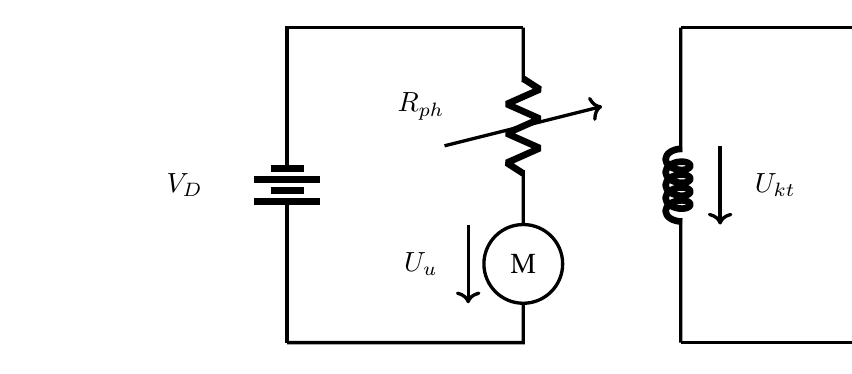
\begin{tikzpicture}
		\begin{circuitikz}
			\drawe (0,0) to [battery] (0,4) to [short] (3,4);
			\draw (-1.3,2) node {$V_{D}$};
			\drawe (3,1.5) to [R] (3,4);
			\drawe[->] (2,2.5) -- (4,3);
			\drawe (3,1) circle (.5) node{M};
			\drawe[->] (2.3,1.5) -- (2.3,0.5);
			\draw (1.7,3) node {$R_{ph}$};
			\draw (1.7,1) node {$U_u$};
			\drawe (3,0.5) to [short] (3,0) to [short] (0,0);
			
			\drawe (5,0) to [short] (8,0) to [battery] (8,4) to [short] (5,4);
			\drawe (5,0) to [L] (5,4);
			\drawe[->] (5.5,2.5) -- (5.5,1.5);
			\draw (6.2,2) node {$U_{kt}$};
			
		\end{circuitikz}
	\end{tikzpicture}
\end{frame}

\begin{frame}{Dùng nguồn cố định kết hợp biến trở}
	\vspace{-.5cm}
	\begin{center}
		\begin{tikzpicture}
			\drawe[->] (0,0) -- (0,3.5);
			\drawe[->] (0,0) -- (8,0);
			
			\drawe[red] (1,0) -- (1,3.5);
			\drawe[magenta] (3,0) -- (3,3.5);
			\drawe[dashed, magenta] (5.5,0) -- (5.5,2.5);	
			
			
			\drawe[draw=blue,-triangle 90,fill=blue] (5.5,0) -- (4.25,0.75);
			\drawe[blue] (4.25,0.75) -- (3,1.5);
			\draw[blue, dashed, line width=.6pt] (3,1.5) -- (0,3);
			
			\drawe[draw=blue,-triangle 90,fill=blue] (3,1.5) -- (4.25,1.5);
			\drawe[blue] (4.25,1.5) -- (5.5,1.5);
			
			\drawe[draw=blue,-triangle 90,fill=blue] (5.5,1.5) -- (4.25,1.9);
			\drawe[blue] (4.25,1.9) -- (3,2.3);
			\draw[blue, dashed, line width=.6pt] (3,2.3) -- (0,3);
			
			\drawe[draw=blue,-triangle 90,fill=blue] (3,2.3) -- (4.25,2.3);
			\drawe[blue] (4.25,2.3) -- (5.5,2.3);
			
			\drawe[draw=blue,-triangle 90,fill=blue] (5.5,2.3) -- (4.25,2.6);
			\drawe[blue] (4.25,2.6) -- (3,2.8);
			\drawe[draw=blue,-triangle 90,fill=blue] (3,2.8) -- (2,2.9);
			\drawe[blue] (2,2.9) -- (0,3);
			\drawe[red, fill=red] (1,3) circle (.1);
			
			\draw (-1,3.3) node {$\omega_m$};
			\draw (-.5,0.3) node {$0$};
			\draw (1,-.5) node{$\textcolor{red}{M_{c}}$};
			\draw (3,-.5) node{$\textcolor{magenta}{M_{min}}$};
			\draw (5.5,-.5) node{$\textcolor{magenta}{M_{max}}$};
			\draw (7.3,-.5) node{$M$};
		
			\draw (6.8,0.5) node {\small{$1 \quad R_{ph_{2}}$}};
			\draw (6.8,1.5) node {\small{$3 \quad R_{ph_{1}}$}};
			\draw (7.3,2.5) node {\small{$5 \quad R_{ph} = 0$}};
			\draw (4,3.3) node {\textcolor{blue}{\small{\text{\textit{đtctn}}}}};
			
			\draw (2.6,1.3) node {\small{$2$}};
			\draw (2.6,2.3) node {\small{$4$}};
			\draw (1.4,3.3) node {\textcolor{red}{\small{$6$}}};
		\end{tikzpicture}
	\end{center}
\end{frame}

%--------------------------------------------------------------------------------
% Khởi động ĐC DC kích từ nối tiếp
\subsection*{Khởi động ĐC DC kích từ nối tiếp}
\begin{frame}{Khởi động động cơ DC kích từ nối tiếp}	
	\begin{itemize}
	\justifying
		\item Khởi động bằng điện trở phụ.
		\item Khởi động bằng cách thay đổi nguồn áp. 
	\end{itemize}
\end{frame}

\begin{frame}{Dùng điện trở phụ}
	\begin{center}
	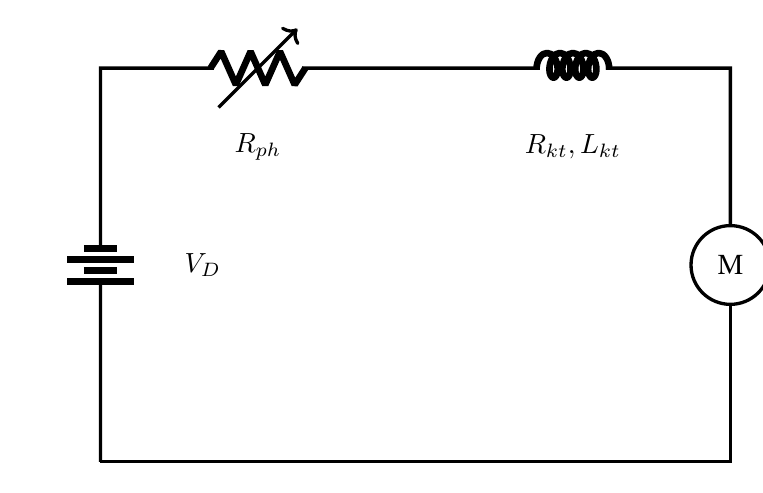
\begin{tikzpicture}
		\begin{circuitikz}
			\drawe (0,0) to [battery] (0,5) to [R] (4,5) to [L] (8,5) to [short] (8,3);
			\drawe[->] (1.5,4.5) -- (2.5,5.5);
			\drawe (8,2.5) circle (.5) node{M};
			\drawe (8,2) to [short] (8,0) to [short] (0,0);
			\draw (2,4) node {$R_{ph}$};
			\draw (6,4) node {$R_{kt}, L_{kt}$};
			\draw (1.3,2.5) node {$V_{D}$};
		\end{circuitikz}
	\end{tikzpicture}
	\end{center}
\end{frame}

\begin{frame}{Dùng điện trở phụ}
\vspace{-.5cm}
\begin{center}
	\includegraphics[scale=.8]{images-chude4/khongdong-kichtu-noitiep-1-2.png} 
\end{center}
\end{frame}

\begin{frame}{Dùng nguồn áp thay đổi}
	\begin{center}
	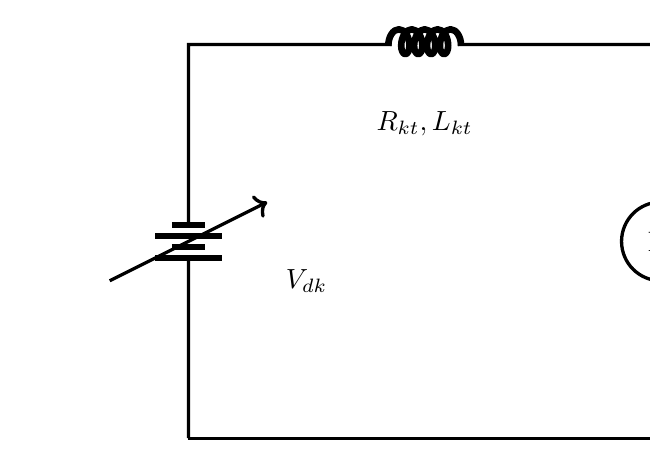
\begin{tikzpicture}
		\begin{circuitikz}
			\drawe (0,0) to [battery] (0,5) to  [L] (6,5) to [short] (6,3);
			\drawe[->] (-1,2) -- (1,3);
			\drawe (6,2.5) circle (.5) node{M};
			\drawe (6,2) to [short] (6,0) to [short] (0,0);
			\draw (3,4) node {$R_{kt}, L_{kt}$};
			\draw (1.5,2) node {$V_{dk}$};
		\end{circuitikz}
	\end{tikzpicture}
	\end{center}
\end{frame}

\begin{frame}{Dùng nguồn áp thay đổi}
\vspace{-.3cm}
\begin{center}
	\includegraphics[scale=.75]{images-chude4/khongdong-kichtu-noitiep-2-1.png} 
\end{center}
\end{frame}

%--------------------------------------------------------------------------------
%--------------------------------------------------------------------------------
% Tài liệu tham khảo
\section*{Tài liệu tham khảo}
\begin{frame}{Tài liệu tham khảo}
%\begin{small}
\justifying
[1]. Nguyễn Văn Nhờ, \textit{Cơ sở Truyền động điện}, NXB ĐH Quốc gia HCM.

[2]. \href{https://www.youtube.com/watch?v=LAtPHANEfQo}{DC Motor, How it works?}
% Video Vietsub: https://www.youtube.com/watch?v=kfClbX_bE1s
%http://ubuntuhandbook.org/index.php/2014/04/install-adobe-reader-ubuntu-1404/
%\end{small}
\end{frame}
%--------------------------------------------------------------------------------
%--------------------------------------------------------------------------------
% Lời cảm ơn
\section*{Lời cảm ơn}
\begin{frame}
\justifying
\large \alert{Cảm ơn Thầy và các bạn đã quan tâm theo dõi phần trình bày của nhóm!}
\end{frame}
\end{document}